% section | subsection | subsubsection | paragraph | subparagraph | verbatim | enumerate | item

% Just let it be an Article bro
\documentclass{article}

% Cover Metadata
\title{Database Clients}
\date{06 Nov 2025}
\author{Maulana Hafidz Ismail}

% Equation Setup
\usepackage{amsmath}

% Image Setup
\usepackage{graphicx}
\usepackage{float}

% Link Setup
\usepackage{hyperref}

% Highlighting Setup
\usepackage{soul}
\usepackage{xcolor}
\sethlcolor{red!30}
\newcommand{\hlblue}[1]{\sethlcolor{cyan!30}\hl{#1}\sethlcolor{yellow}}

% Line Width
\sloppy
\setlength{\emergencystretch}{3em}
\hbadness=99999

% Code Syntax Setup
\usepackage{listings}
\usepackage{xcolor} % untuk warna
\lstset{
basicstyle=\ttfamily\small,
frame=single,
breaklines=true,
backgroundcolor=\color{gray!10},
keywordstyle=\color{blue},
commentstyle=\color{gray},
stringstyle=\color{red},
tabsize=2,
captionpos=b
}

% Start of the Article
\begin{document}

% Cover Page
\pagenumbering{gobble}
\maketitle
\newpage

% Table of Content Page
\tableofcontents
\newpage
\pagenumbering{arabic}

% Main Content
\section{Interacting with a MySQL database using Python}
\subsection{Database Clients}
MySQL adalah sistem manajemen basis data SQL sumber terbuka. Ini adalah basis data relasional yang menyimpan data dalam tabel-tabel terpisah. Perangkat lunak basis data MySQL mengikuti sistem client/server, dan server dapat dijalankan di desktop atau laptop tanpa memerlukan pengawasan yang signifikan. MySQL cepat, andal, skalabel, dan mudah digunakan.

Sistem klien/server MySQL terdiri dari server SQL yang mendukung berbagai program klien dan antarmuka pemrograman aplikasi (API) untuk mengelola basis data.

Dalam sistem client/server, MySQL sebagai server basis data adalah perangkat lunak yang berfungsi sebagai backend tempat Anda dapat membuat dan menyimpan basis data. Sedangkan client adalah perangkat lunak yang dapat Anda gunakan untuk terhubung ke server basis data MySQL guna melakukan operasi yang diperlukan menggunakan kueri SQL pada basis data. Client memungkinkan Anda untuk mengintegrasikan basis data MySQL ke dalam aplikasi Anda.

Database MySQL dirancang untuk bekerja dengan berbagai perangkat lunak, program, dan bahasa pemrograman. Semua perangkat lunak tersebut memiliki klien khusus untuk berinteraksi dengan database, dan klien-klien ini juga disebut driver atau API.

\begin{figure}[H]
    \centering
    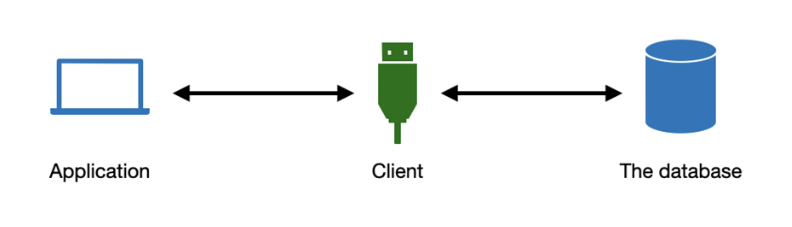
\includegraphics[width=0.8\textwidth]{./Picts/clients.png}
    \caption{}
\end{figure}

\newpage


\section{Performing Queries in MySQL using Python}


\newpage


\section{Advanced Database Clients}


\newpage


\section{Working with a Database Client}




% End of Main Content
\end{document}